\documentclass[12pt,epsf,psfig,graphics]{article}             
\textwidth = 6.5in
\textheight = 9.05in
\topmargin 0.0in
\oddsidemargin 0.0in
\evensidemargin 0.0in

% set it so that subsubsections have numbers and they
% are displayed in the TOC (maybe hard to read, might want to disable)

\usepackage[T1]{fontenc}
\usepackage{mathptmx}

\usepackage{epsfig}

%\usepackage{graphics}

\setcounter{secnumdepth}{3}
\setcounter{tocdepth}{3}

% define widow protection 
        
\def\widow#1{\vskip #1\vbadness10000\penalty-200\vskip-#1}

% define a little section heading that doesn't go with any number

\def\littlesection#1{
\widow{2cm}
\vskip 0.5cm
\noindent{\bf #1}
\vskip 0.1cm
\noindent
}

% A paraphrase mode that makes it easy to see the stuff that shouldn't
% stay in for the final proposal

\newdimen\tmpdim
\long\def\paraphrase#1{{\parskip=0pt\hfil\break
\tmpdim=\hsize\advance\tmpdim by -15pt\noindent%
\hbox to \hsize
{\vrule\hskip 3pt\vrule\hfil\hbox to \tmpdim{\vbox{\hsize=\tmpdim
\def\par{\leavevmode\endgraf}
\obeyspaces \obeylines 
\let\par=\endgraf
\bf #1}}}}}

\renewcommand{\baselinestretch}{1.2}    % must go before the begin of doc
\newtheorem{principle}{Principle}
\newtheorem{definition}{Definition}
\newtheorem{define}{Definition}
% go with the way that CC sets the margins

\begin{document}

% handle widows appropriately
\def\widow#1{\vskip #1\vbadness10000\penalty-200\vskip-#1}

\begin{center}

CS290: Principles of Software Development \\
Final Examination \\
%Saturday December 11, 2004 \\

\end{center}

\noindent
Answer the ten questions that are listed on the following pages.  You
must provide answers to these questions on a separate sheet of paper.
Please develop responses that clearly express your ideas in the most
succinct manner possible.  You are not permitted to complete this
examination in conjunction with any of your classmates.  Furthermore,
you cannot consult any outside references during this examination.  If
you have questions concerning the problems that are given below, then
please visit my office during the examination period.  If you leave
the classroom to take the exam, then you are responsible for checking
the white board for status updates.

%\mbox{} \newline
%\mbox{} \newline

\begin{enumerate}
  
\item ({\bf 10 Points}) In {\em The Mythical Man Month} Frederick
  Brooks states that there is no {\em silver bullet} for the field of
  software engineering.  That is, he believes that there is no
  technical or managerial development that will offer an order of
  magnitude improvement in productivity. In order to support his
  argument, Brooks describes several concepts in light of the
  productivity equation provided in Equation~\ref{productivity}.

        \begin{equation} \label{productivity}
        \mbox{{\em Time of software project}} = \sum_{i = 1}^{n} 
                \mbox{{\em Frequency}}_i \times \mbox{{\em Time}}_i
        \end{equation}

        \begin{center}
          for tasks $t_1, \ldots, t_n$
        \end{center}

        \begin{enumerate}
          
        \item ({\bf 4 Points}) Explain the notions of {\em essence}
          and {\em accident} as Frederick Brooks defines them in the
          {\em Mythical Man Month}.  Give one or two examples of each
          concept.
          
        \item ({\bf 2 Points}) Using Equation~\ref{productivity},
          explain why Brooks asserts that there is no silver bullet to
          solve the problems that are associated with constructing
          software.
        
        \item ({\bf 2 Points}) Brooks states that software engineers
          have developed a number of potential silver bullets.
          Discuss two candidates for silver bullets and state whether
          or not you believe that they are indeed silver bullets.

        \item ({\bf 2 Points}) The NATO Software Engineering
          Conferences, held in 1968 and 1969, were the first to define
          the term ``software engineering.''  What does this term
          mean?

       \end{enumerate}
        
\newpage

\item ({\bf 10 Points}) Software process models are used as
  abstractions that can help to explain different approaches to
  software development. Respond to the following questions about how
  process models can guide the creation of software systems.

        \begin{enumerate}
          
        \item ({\bf 4 Points}) Discuss the fundamental ``phases'' that
          are common to most software processes and furnish a one or
          two sentence description of each activity.  Please include
          an example of one or two tools that can support each of
          these activities. If no tool support is available, then
          clearly state why this is the case!  Your response should
          include a properly labeled figure that includes the phase
          and its input and output.
          
%%         \item ({\bf 2 Points}) After clearly explaining the halting
%%           problem, select one phase of the software lifecycle and
%%           discuss how the halting problem is relevant to an activity
%%           in this phase.

        \item ({\bf 2 Points}) {\em Agile software development} (or,
          {\em extreme programming}) is a software process model based
          on iteration.  What are the most relevant features of this
          approach to organizing the phases of the software lifecycle?

        \item ({\bf 2 Points}) Explain the similarities and
          differences between the waterfall lifecycle model (i.e., the
          ``traditional'' model that Pfleeger and Atlee initially
          describe in Chapter 2) and the spiral model proposed by
          Boehm.

        \item ({\bf 2 Points}) An {\em activity graph} $G = \langle N,
          E \rangle$ can be used to manage the developers in a
          software project.  How does the {\em critical path method}
          (CPM) use activity graph $G$ to support project management?
          Beyond explaining the CPM, your response to this question
          should correctly define the two components of $G$.

        %% \item ({\bf 2 Points}) A node in an activity graph stands for
        %%   a task or milestone in a software development project.  What
        %%   is the meaning behind the nodes and edges in an activity
        %%   graph when they have the following two configurations?

        %%   \begin{enumerate}

        %%     \item Nodes $N_i$ and $N_j$ that are connected by a
        %%       directed and solid edge from $N_i$ to $N_j$

        %%     \item Nodes $N_k$ and $N_l$ that are connected by a
        %%       directed and dashed edge from $N_k$ to $N_l$

        %%   \end{enumerate}

        \end{enumerate}

\newpage

\item ({\bf 10 Points}) Hamlet and Maybee outline several suggestions
  for the creation of a high quality requirements document.  Answer
  the following questions about the requirements elicitation and
  analysis phase of the software lifecycle.

%% It is difficult to write a requirements document that adheres to the
%% IEEE Standard for a {\em software requirements specification} and
%% contains individual requirements that uphold the regulations
%% established by Hamlet and Maybee.

        \begin{enumerate}

        \item ({\bf 4 Points}) For each of the following requirements,
          you should state whether they exhibit the properties of good
          requirements and then explain why you made this judgment.
          If you determine that the requirement is poorly written,
          then you must furnished an improved restatement of the same
          functionality.

          \begin{enumerate}

            \item ({\bf 2 Points}) ``We feel that good systems provide
              the end user with good value.  Because of this, we think
              that the system should provide adequate performance with
              a 2 Gb disk, since this is the least expensive disk that
              we may purchase from the designated vendor.  Of course,
              the user may elect to configure the system with a larger
              disk, and we recommend this, but we have attempted to
              come to grips with most of the problems raised by use of
              a smaller disk, and we feel that they can be, by and
              large, satisfactorily resolved.''

            \item ({\bf 2 Points}) ``The system shall accept valid
              employee ID numbers from 1 to 9999.''

          \end{enumerate}                    
          
        \item ({\bf 3 Points}) Hamlet and Maybee stress that
          requirements should be {\em non-prescriptive} in nature.
          After defining what this term means, please provide an
          example of a requirement that is non-prescriptive and
          another that fails to adhere to this standard.  Your
          response to this question should not use either of the two
          previous requirements.

        \item ({\bf 3 Points}) Suppose that you are part of a
          development team that is responsible for implementing a
          compiler for the Java programming language.  The manager of
          your team asks you to fully implement {\em array-bounds
            checking} in your compiler.  After defining what this term
          means, explain whether or not this requirement is {\em
            feasible}.

        \end{enumerate}

\newpage

\item ({\bf 10 Points}) Managers often use a software process in order
  to make decisions about when to release an application.  For
  example, suppose that you are a manager and you are determining
  which features will be a part of the next release of your program.
  Moreover, assume that for each new requirement $R_j$ you already
  know $C_j$, the cost associated with implementing the requirement
  and $B_j$, the monetary benefit for a program that contains this
  feature.

  In order to determine which requirements will be part of the next
  release for your application, you must choose from the requirements
  $R = \{ R_1, \ldots, R_n \}$ and ensure that (i) the implementation
  tasks are completed at no more than the total fixed cost $C$ and
  (ii) you maximize the total monetary benefit that your company will
  see when they release the tool.  Given cost and benefit information
  for each $R_j$ and the fixed cost $C$, how will you determine which
  requirements are included in the next release of your program?
    
\newpage

\item ({\bf 10 Points}) Research in software architectures has flourished
in recent years.  Answer the following question about software architectures
by providing a response for each part.

\begin{enumerate}

\item ({\bf 2 Points}) Define the term {\em software architecture}.
  Discuss some of the advantages that are associated with explicitly
  designing and documenting a software architecture.  Your response
  should include the name of a software architecture that is different
  than the two mentioned in the later parts of this question and the
  question on the next page.

\item ({\bf 4 Points}) The {\em shared repository} model (or, {\em
  blackboard}, or {\em tuple space}) is one example of a software
  architecture.  After explaining the features of this architecture
  and providing an explanatory diagram, discuss at least one strength
  and one weakness of this model for structuring a software system.
  Your response should provide an example of a software application
  that could potentially adhere to this architecture.

\item ({\bf 2 Points}) The {\em pipe and filter} is another example of
  a software architecture.  In this architecture, filters are
  processing units that are connected with pipes.  Discuss at least
  one strength and one weakness of this type of software architecture.
  You should use Unix pipes and filters as a frame of reference for
  your response.

\item ({\bf 2 Points}) Figure~\ref{fig:ps} gives a diagram that
  illustrates the {\em publish/subscribe} architecture.  Using this
  schematic as the main reference for this architecture, completely
  describe the features and operation of a software system that
  adheres to this approach to structuring an application.  What are
  the strengths and weaknesses of your system?

\end{enumerate}

\begin{figure}[h]
\begin{center}
%\vspace*{-.15in}
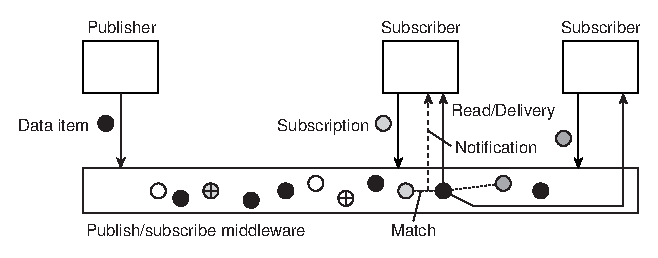
\includegraphics{13-02.eps}
\end{center}
\vspace*{-.2in}
\caption{A Diagram of the Publish/Subscribe Architecture.}
\vspace*{-.15in}
\label{fig:ps}
\end{figure}

\newpage

\item ({\bf 10 Points}) It is important to pick the right architecture
  and design for a software application.  Answer the following
  questions about software architecture and design.

\begin{enumerate}

\item ({\bf 2 Points}) The Object Management Group (OMG) defined
  something called the {\em unified modeling language} (UML).  What is
  the UML?  Your response to this question should give two examples of
  diagrams that you can construct with the UML.

\item ({\bf 2 Points}) The authors of the book {\em The Pragmatic
  Programmer: From Journeyman to Master} suggest that software
  developers should follow these two tips.  What do these tips mean?
  What are the efficiency and effectiveness trade-offs associated with
  engineering software applications that adhere to these rules?

  \begin{enumerate}

  \item Tip: Minimize Coupling Between Modules

  \item Tip: Put Abstractions in Code, Details in Metadata

  \end{enumerate}

\item ({\bf 2 Points}) For the final project in this course, you
  implemented Maxwell, a heat loss and gain calculator.  Please draw
  one or more diagrams to represents the architecture and design of
  this software system.

\item ({\bf 4 Points}) Figure~\ref{fig:cs} gives a diagram that
  illustrates the {\em client/server} architecture at use in a network
  file system (NFS).  Using this schematic as the main reference for
  this architecture, please give a detailed explanation of two
  strengths and two weaknesses of a file system that operates in a
  client/server fashion.

\end{enumerate}

\begin{figure}[h]
\begin{center}
%\vspace*{-.15in}
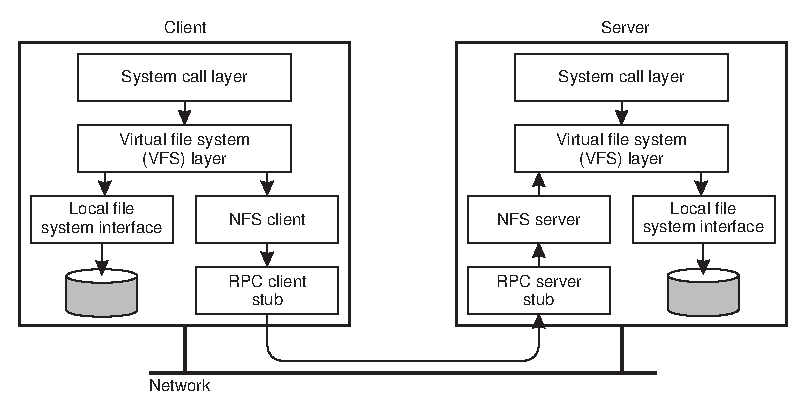
\includegraphics{11-02.eps}
\end{center}
\vspace*{-.2in}
\caption{A Diagram of the Client/Server Architecture.}
\vspace*{-.15in}
\label{fig:cs}
\end{figure}

\newpage

\item ({\bf 10 Points}) Defect testing is focused on finding the
  ``bugs'' in a program.  In order to isolate a defect, a test input
  must execute the defect, infect the data state, and propagate to the
  program's output.  Answer the following questions about defect
  testing and use the code segment in Figure~\ref{pie_code} to answer
  Part~\ref{need_code}.

\begin{figure}[h]

\footnotesize{
\begin{verbatim}
        /* This program is supposed to calculate the velocity of an
           object based upon its kinetic energy and its mass. */
        main() 
        {
          int velocity, velocity_squared, mass, kinetic = 1;
          if( kinetic != 0 ) 
          {
            printf(``Enter Kinetic Energy and Mass of Object:'');
            scanf(``%d %d'', &kinetic, &mass);
            if( mass != 0 ) 
            {
        [*]   velocity_squared = 3 * (kinetic / mass);
              velocity = sqrt(velocity_squared);
              printf(``The Velocity is: %d'', velocity); 
            }
            else 
            {
              printf(``The Velocity is Undefined.\n'');
            }
          }
        }
\end{verbatim} }

\vspace*{-.2in}

\caption{Program that Should Calculate the Velocity of an Object.}
\label{pie_code}
\end{figure}

\begin{enumerate}

\item \label{need_code} ({\bf 10 Points}) The general formula for
  calculating the kinetic energy of an object is \(
  kinetic=\frac{1}{2}mass\times velocity^2 \).  Thus, the equation for
  the {\tt velocity} variable should be \( velocity=sqrt(2 \times
  (kinetic / mass)) \).  At the {\tt [*]} position inside of the code,
  we see that the calculation for {\tt velocity\_squared} includes a
  $3$ instead of a $2$.  Using the following scenarios, describe the
  execution of the program in Figure~\ref{pie_code}.  Make sure that
  you clearly state whether the provided inputs will isolate the
  defect located at the {\tt [*]} position inside of the C source
  code.

%\newpage

\begin{itemize}

\item Scenario 1: input 5 0
\item Scenario 2: input 0 5
\item Scenario 3: input 1000 5
\item Scenario 4: input 8 1

\end{itemize}

\end{enumerate}

\newpage

\item ({\bf 10 Points}) Testing is a part of the software lifecycle
  that can be used for many different purposes.  Provide a response 
  to each of the following questions about testing.

\begin{enumerate}       
  
\item ({\bf 2 Points}) Pfleeger and Atlee identify different types of
  activities such as unit, integration, and system testing.  What is
  the motivation behind performing these tasks?

%% \item ({\bf 2 Points}) Software testing is useful because of the
%%   benefits that you enumerated in response to the first part of this
%%   question.  Yet, testing has several different limitations.  Discuss
%%   two of the limitations commonly associated with software testing.

\item ({\bf 2 Points}) Software engineers often measure the {\em
  complexity} of the software application in order to make decisions
  during the implementation, testing, and maintenance phases.  After
  defining the terms {\em cyclomatic complexity} and {\em
    non-commented source statements}, please explain how to use these
  metrics during the aforementioned phases.
  
\item ({\bf 2 Points}) What are the similarities and differences
  between the implementation and testing of hardware and software?  Is
  it easier to test hardware or software?  Why?

\item ({\bf 4 Points}) {\em Verification} and {\em validation} are two
  activities that software engineers commonly perform during the
  construction of a software application.  In your response to this
  part of the question, please define both of these terms and for each
  term furnish a concrete example of an associated activity.
  
\end{enumerate}

\newpage

\item ({\bf 10 Points}) The implementation and testing phases of the
  software lifecycle enable software engineers to create real, working
  systems.  Answer the following questions about the implementation
  and testing of software.

\begin{enumerate}

  \item ({\bf 2 Points}) What is the meaning of the terms {\em fault}
    and {\em failure}?

  \item ({\bf 2 Points}) One guideline for implementing a high-quality
    software application is to ``localize the input and the output.''
    What is the meaning of this guideline?  Your response to this
    question should also clearly explain whether you followed this
    guideline during the implementation of your final project.

  \item ({\bf 2 Points}) Software testing is traditionally seen as
    having two distinct purposes.  Please state and define the two
    purposes of software testing.

  \item ({\bf 4 Points}) It is possible to divide all of the faults
    found in a software application into two different categories --
    what are they?  After defining each fault category, your response
    to this question should suggest a type of analysis or testing that
    can find and resolve each type of software fault.

\end{enumerate}

%% \item ({\bf 10 Points}) Mutation testing has emerged as one technique
%%   that can be used during the verification and validation process.
%%   Answer the following question about mutation testing and use the
%%   definitions below to respond to Part~\ref{compare}.

%% \begin{define}

%% If P is a program to implement function F on domain D, then a test set
%% T $ \subset $ D is adequate for P and F if ( $\forall$ programs Q ),
%% $[Q(D) \neq F(D) ] \Rightarrow [(\exists t \in T) (Q(t) \neq F(t))]$.

%% \label{adeq}
%% \end{define}

%% \begin{define}

%% If P is a program to implement function F on domain D and $\Phi$ is a
%% finite collection of programs, then a test set T $ \subset $ D is
%% adequate for P relative to $\Phi$ if ( $\forall$ programs Q $\in \Phi$
%% ), $[Q(D) \neq F(D) ] \Rightarrow [(\exists t \in T) (Q(t) \neq
%%   F(t))]$.

%% \label{rel}
%% \end{define}

%% \begin{enumerate}

%% \item \label{compare} ({\bf 3 Points}) Definitions~\ref{adeq} and
%%   \ref{rel} provide a description of the terms {\em adequate} and {\em
%%     relative adequate}.  Using these definitions, explore the
%%   similarities and differences between the terms adequate and relative
%%   adequate.  How are these definitions related to the application of
%%   mutation testing to a Java program $P$ and a JUnit test suite $T$?

%% \item \label{purpose} ({\bf 3 Points}) Explain the main reason for
%%   performing mutation testing. Next, suppose that a given test suite
%%   is able to kill $80\%$ of the syntactic mutants in the set $\Phi$.
%%   Discuss how this could influence the remainder of the testing
%%   effort.

%% \item ({\bf 2 Points}) Suppose that you are developing a mutation
%%   testing tool for relational operators.  If your tool encountered the
%%   statement {\tt if(num\_deposits > MAX\_DEPOSITS)}, what syntactic
%%   mutants would you generate to populate the set $\Phi$?

%% \item ({\bf 2 Points}) Mutation testing can be a very powerful
%%   technique during verification and validation.  However, it also has
%%   several important limitations.  Discuss two or three of the major
%%   limitations of mutation testing.  Your response should provide the
%%   name of one or two mutation testing tools that are available for the
%%   Java programming language.

%% \end{enumerate}

\newpage

\item ({\bf 10 Points}) Software implementation is the process of
  translating the software specification, design, and architecture
  into an executable representation.  Answer the following questions
  about the implementation and evaluation of computer software.

\begin{enumerate}

  \item ({\bf 3 Points}) Implement a data generator that takes a list
    of numbers as input and then produces a list of lists as output.
    For instance, please consider the following outputs for the input
    list 1 2 3 4.  From this example, you can see that the data
    generator must return all of the lists that may be obtained by
    swapping certain items in the input list.  In this specific
    instance, an input list of size four produces an output list that
    contains six individual lists.  You may implement your data
    generator in any programming language.

    \begin{enumerate}

    \item 2 1 3 4
      
    \item 3 2 1 4

    \item 4 2 3 1

    \item 1 3 2 4
        
    \item 1 4 3 2

    \item 1 2 4 3

  \end{enumerate}

  \item ({\bf 3 Points}) Provide a test plan for the data generator
    that you implemented in Part 10a of this question.  Your plan
    should identify the inputs and anticipated output for each of the
    tests.  You should also clearly explain why you decided to include
    each of the test cases into the overall plan.

  \item ({\bf 2 Points}) Jeffrey Voas poses the question ``can clean
    pipes produce dirty water?'' in an article of the same title from
    IEEE Software.  What is the meaning behind the concepts of ``clean
    pipes'' and ``dirty water''?  In the context of software
    engineering, what is your response to the question raised by Voas?

  \item ({\bf 2 Points}) Software engineers commonly ask themselves
    the question ``when should we stop testing our software?''  Please
    fully explain two valid responses to this question.

  %% \item ({\bf 2 Points}) The software engineers at Google recently
  %%   found a defect in the traditional implementation of the binary
  %%   search.  What was the defect in this algorithm?  Your response to
  %%   this question should clearly explain the situation(s) in which
  %%   this fault would manifest itself as a failing execution of a Java
  %%   program.

\end{enumerate}

\end{enumerate}

\end{document}
